\iffalse
\bibliography{reference/refs}
\fi


\chapter{Proposed Methodology}

Procrustes analysis, named after a bandit from Greek mythology who streches or cut off his victim to his bed, is used to analyse the distribution of a set of shapes. Shape is all geometrical information that remains when location, scale and rotational effects are filtered out from an object ~\cite{IMM2002-0403}. 

For ASM (Active Shape Model), the training data set contains arbitrary size images for the Procrustes analysis would normalize the data.

Why do I use tensor decomposition to do the face de-identification? Firstly, model-based approach is a good way to protect privacy. The weakness of it is about the data utility. Is it possible to decompose the face images into several dimensions with each one containing one kind of information? Data is always represented as vector, order-1 tensor. Tensor is a multi-dimensional array. It is designed to represent multi-dimensional data. We can regard a face image as a tensor which contains multidimensional informations. Our work is just to decompose it and pick the informations out. 

Diagram of the method

\begin{figure}
  \centering
  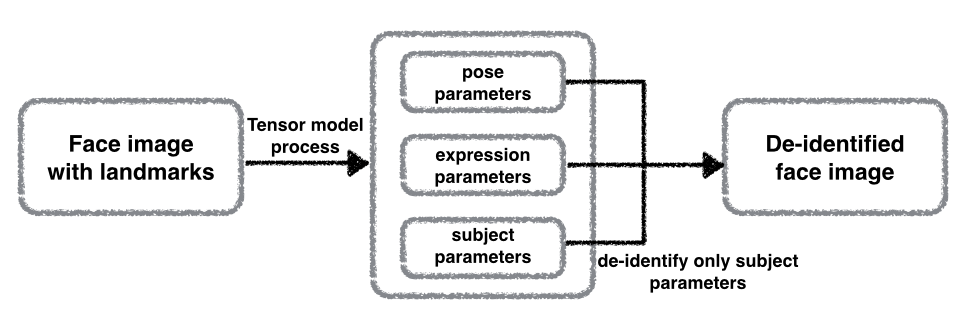
\includegraphics[width=0.99\textwidth]{figure/diagram} 
  \caption{The whole process}
  \label{diagram}
\end{figure}


\section{Background Knowledge}
AAM (Active Appearance Model)


\section{Method}

They proposed a linear mapping that is intuitive given the nature of the vectors that span shape and appearance space of AAM. Each component of a shape vector is an offset of the mean shape, the same as appearance. Also the vector itself represents the overall displacement that gives rise to a specific type of gesture (Add a picture? ). One vector might be responsible for opening and closing the mouth, while another might control eye blink, and so on. ~\cite{Theobald07}

However, it is far more complex in real situations. Multiple vectors control the eye blink. The correspondence between models are different. 



The inverse composition image alignment has its own shortcomings. It still takes a long time to compute for the complex matrix computation in each iteration. On the other hand, the inverse composition algorithm is based on gradient. The algorithm is easily influenced by noise, block, and illuminations. The future work is to improve the speed and robust of inverse composition algorithm. 






		Inspired by ~\cite{Vasi02}, we think that it is possible to decompose a face image into multiple dimensions with each one containing parameters corresponding to specific information. Motivated by the famous active appearance model (AAM) ~\cite{Matthews_04}, we also separate a face image into shape and appearance. The face images used are all with proper landmarks. Based on a tensor model, a face image is decomposed for de-identification. Our proposed basis-based de-identification and percentage-based de-identificaion are applied depending on situations. Before the decomposition, a tensor model should be constructed. 

		To distinguish from scalars, vectors, matrices and higher-order tensors, different symbols are used: scalars are represented by Greek alphabet letter $\alpha,\beta,\lambda,...$ and lower case letters $a,b,c,...$, vectors are denoted by bold lower case letter ${\bf (a,b,c,...)}$, capital letters $(A,B,C,...)$ are for matrices, and tensors are described by calligraphic letters $(\mathcal{A,B,C,...})$. A tensor is denoted by $\mathcal{A} \in R^{I_1 \times I_2 \times ... \times I_N}$, where $N$ is the order of a tensor. $\mathcal{A}$ can be unfolded by stacking its mode-$n$ vectors as columns in a matrix as $A_{(n)} \in R^{I_n \times (I_1I_2...I_{n-1}I_{n+1}...I_N)}$. 

		Firstly, shapes of all training face images are normalized and Procrustes analyzed iterately. After that, appearance of each face would be warped to processed mean shape. We build the data into a tensor $\mathcal{A} \in R^{I_{pose} \times I_{exp} \times I_{id} \times I_{data}}$ where $I_{pose}, I_{exp}, I_{id}$ are the number of pose, expression, identity included in training data. For shape, $I_{data}$ is the twice number of landmarks labeled in a training image because of $points = [x_1,x_2,...,x_n,y_1,y_2,...,y_n]^T$. For appearance, $data$ is usually the vector form of all pixels and $I_{data}$ should have been the number of pixels, but the computation of Higher order singular value decomposition (HOSVD) ~\cite{Lathauwer00} is too slow when training image is large. HOSVD, also called Tucker decomposition, would decompose a tensor $\mathcal{A} \in R^{I_1 \times I_2 \times ... \times I_N}$ into mode-n product of $N$ orthogonal matrices $U_n \in R^{I_n \times I_n}$ and a core tensor $\mathcal{Z} \in R^{I_1 \times I_2 \times ... \times I_N}$: $\mathcal{A} = \mathcal{Z} \times_1 U_1 \times_2 U_2 ... \times_N U_N$. For the given tensor $\mathcal{A}$ and a matrix $M \in R^{J_n \times I_n}$, the mode-n product is denoted as: $(\mathcal{A} \times_n M)_{i_1...i_{n-1}j_ni_{n+1}...i_N} = \sum_{i_n=1}^{I_n}a_{i_1...i_{n-1}i_ni_{n+1}...i_N}*m_{j_ni_n}$.

		It is time-consuming to get the HOSVD result of an appearance tensor, especially when the size of trainning image is getting larger and larger. 2D appearance representation \cite{Feng12} could speed up the computation. For this reason, the HOSVD representation of shape and appearance tensor is built as:

		\begin{equation}
			\mathcal{A}_{s} = \mathcal{Z}_{s\_core} \times_1 U_{s\_pose} \times_2 U_{s\_exp} \times_3 U_{s\_id} \times_4 U_{points}.
		\end{equation}

		\begin{equation}
			\mathcal{A}_{a} = \mathcal{Z}_{a\_core} \times_1 U_{a\_pose} \times_2 U_{a\_exp} \times_3 U_{a\_id} \times_4 U_{px} \times_5 U_{py}.
		\end{equation}
		
		To describe the proposed method in a brief way, the shape and appearance tensors are both written as:
		\begin{equation}
			\mathcal{A} = \mathcal{Z}_{core} \times_1 U_{pose} \times_2 U_{exp} \times_3 U_{id} \times_4 U_{data},
			\label{base_equation}
		\end{equation}
		where $U_{data}$ is $U_{points}$ for shape tensor and $U_{px} \times U_{py}$ for appearance tensor.

		%HOSVD
		\subsection{Basis-based De-identification}

				For a specific $i$th pose and $j$th expression, we can get an image basis subtensor $\mathcal{B}_{i,j}$ using the product of core tensor and the corresponding row of mode-n matrix \cite{TPAMI09}, like:
				\begin{equation}
					\mathcal{B}_{(i,j)} = \mathcal{Z}_{core} \times_1 U_{pose}(i,:) \times_2 U_{exp}(j,:) \times_4 U_{data}.
				\end{equation}
				
				Unfolding $\mathcal{B}_{(i,j)}$ along data dimension, we got a matrix $B(i,j) \in R^{I_{data} \times I_{id}}$. Assume the parameter of identity is ${\bf c_{id}} \in R^{I_{id} \times 1}$, the original input face iamge $data$ can be reconstructed as:
				\begin{equation}
					data = B(i,j) * {\bf c_{id}}.
				\end{equation}
				Therefore, the identity parameters should be:
				\begin{equation}
					{\bf c_{id}} = B(i,j)^{-1} * data.
				\end{equation}

				When the $i$th pose and the $j$th expression are chosen iterately, numbers of {\bf $c_{id}$} are computed. The deviation between original data and reconstructed data, $d_{recon}$, is defined as:
					\begin{equation}
						d_{recon} = ||data - B(i,j)*{\bf c_{id}}||.
						\label{deviation_ij}
					\end{equation}

				After testing all poses and expressions, there must be a pose and expression that minimizes $d_{recon}$. The pose and expression that make $argmin(d_{recon})$ are regarded as the pose and expression of input face image.  

				One face image with identity parameter, ${\bf c_{id\_1}}$, can be de-identifed by computing new image as $B(i,j)*{\bf c_{id\_new}}$. 
				\begin{equation}
					{\bf c_{id\_new}} = \frac{ ({\bf c_{id\_2}} + {\bf c_{id\_1}})}{2},
				\end{equation}
				where ${\bf c_{id\_2}}$ is identity parameter of another face image who wears the same pose and expression as the original one. It is surely feasible to construct ${\bf c_{id\_new}}$ with more face images. 

				Since the data dimension we illustrate contains both appearance and shape, the two results are computed individually. To get the de-identified face image, appearance should be warped back to its corresponding shape.

				So far, the introduced approach is similar to {\it k-Same-Select} while implemented in a much easier way. The basis-based de-identification has the same shortcoming as {\it k-Same-Select}: the weak ability to represent non-trained type of data.

		\subsection{Percentage-based De-identification}
		If the minimum number of Equation.\ref{deviation_ij} is too large or bigger than a pre-defined threshold, it means the type of $data$ is not included in the training set. The decomposition of basis-based approach might be inaccurate when the type of input image is not trained. It is possible to enlarge training dataset to enhance the model representation ability. However,  inspired by "continous variation estimation" ~\cite{TPAMI09}, we come up with the percentage-based de-identification method based on rank-n approximation of a tensor. For a third-mode tensor $\mathcal{A} \in R^{m \times n \times q}$, it can be decomposed into the sum of outer product of three vectors, ${\bf a_i} \in R^{m \times 1}, {\bf b_i} \in R^{n \times 1}, {\bf c_i} \in R^{q \times 1}$ and a scalar $\lambda_i$, by the rank-n approximation (also known as CP decomposition) ~\cite{Lathauwer_rank}: $\mathcal{A} = \sum_{i=1}^{n}\lambda_i \circ {\bf a_i} \circ {\bf b_i} \circ {\bf c_i}$ where $\circ$ indicates outer product. 

		Since the pose and expression of input image are not included in training data set, ${\bf c_{pose},c_{exp},c_{id}}$ are supposed to be its parameters in pose, expression and identity dimensions. According to Equation.~\ref{base_equation}, the original data should be:
		\begin{equation}
			\begin{aligned}
				data & = \mathcal{Z}_{core} \times_1 ( {\bf c_{pose}^T} * U_{pose} ) \times_2 ({\bf c_{exp}^T} * U_{exp}) \\ & \times_3 ({\bf c_{id}^T} * U_{id}) \times_4 U_{data} \\
				& = \mathcal{A} \times_1 {\bf c_{pose}^T} \times_2 {\bf c_{exp}^T} \times_3 {\bf c_{id}^T} \\
				& = A(data) * {\bf c_{para}}, \\
			\end{aligned}
		\end{equation}
		where $A(data) \in I_{data}\times I_{pose*exp*id}$ is the unfolding matrix of $\mathcal{A}$ along $data$ dimension and ${(\bf c_{para}} = {\bf c_{pose}} \otimes {\bf c_{exp}} \otimes {\bf c_{id}}) \in I_{pose*exp*id} \times 1$, thus:
		
		\begin{equation}
			{\bf c_{para}} = A_{(data)}^{-1} * data,
		\end{equation}
		for which the {\it F-Nearest Equation Construction} strategy \cite{lin05} is used to get an unique solution for ${\bf c_{para}}$. 
		
		Our purpose is to get the individual parameters in each dimension rather than the combination parameters. Regarding ${\bf c_{para}}$ as a tensor, the best rank-1 approximation ~\cite{Lathauwer_rank} could be used to decompose ${\bf c_{para}}$ properly. The tensor can be represented as a scalar times outer product of three vectors. However, our experiment indicates that the rank-1 approximation has a large deviation with the original data. Rank-n approximation would get almost perfect reconstruction of original parameters when the $n$ is large, written as:

		\begin{equation}
			{\bf c_{para}} = \sum_{i=1}^{n}\lambda_i {\bf c_{pose}^i} \otimes {\bf c_{exp}^i} \otimes {\bf c_{id}^i}
		\end{equation}
		
		The reconstructed data by ${\bf c_{para}}$ is:
		\begin{equation}
			\begin{aligned}
				recon\_data & =A_{(data)} * {\bf c_{para}} \\
				& = A_{(data)} * \sum_{i=1}^{n}\lambda_i {\bf c_{pose}^i} \otimes {\bf c_{exp}^i} \otimes {\bf c_{id}^i} \\
				& = \sum_{i=1}^{n}A_{(data)} * {\bf c_{para}^i}, \\
			\end{aligned}
		\end{equation}
		where ${\bf c_{para}^i} = \lambda_i {\bf c_{pose}^i} \otimes {\bf c_{exp}^i} \otimes {\bf c_{id}^i}$ and $recon\_data$ can be seen as a combination of $n$ sub-images data. Each of these sub-images contains three dimension parameters: pose, expression and identity. Percentage of the $i$th sub-image,$p_i$, in original image is:
		\begin{equation}
			p_i = \frac{\lambda_i}{\sum_{i=1}^{n}\lambda_i}.
		\end{equation}

		Based on percentages, we can select the sub-images to replace the original identity parameters.	The de-identified image can be described as:
		\begin{equation}
			\begin{aligned}
				recon\_data & = A_{(data)} * (\sum_{i=1}^{m}\lambda_i {\bf c_{pose\_1}^i} \otimes {\bf c_{exp\_1}^i} \otimes {\bf c_{id\_1}^i} \\ & + \sum_{j=m+1}^{n}\lambda_j {\bf c_{pose\_1}^j} \otimes {\bf c_{exp\_1}^j} \otimes {\bf c_{id\_new}^j}),
			\end{aligned}
			\label{compo}
		\end{equation}
		where $1<m<n$ and ${\bf c_{id\_new}}$ is identity parameters from another subject. The effectiveness of reconstruction results change depending on the value $m$. Similarity between subjects can be estimated by equation \ref{deviation_ij}. 
